\section{实验验证}
\label{sec:experiment}

\subsection{实验协议}

实验基于同一套 Apollo 风格路径--速度规划链比较四种方法：B0 为时间盲固定裕度与逐障碍物贪心选向；B1 加入到达时间投影，但仍使用单一空间选向；B2 采用路径--速度迭代更新到达时间；MIKU 启用鲁棒占据、差异化裕度、分组连续分割、Top-K 空间候选、时间同伦图、双向 ST 约束与按需细化。所有方法共享车辆尺寸、道路边界、预测输入、路径/速度 QP、动力学界和目标权重，从而把差异集中在时空约束组织方式上。

主实验包含行人横穿、车辆切入、停车车辆与对向车、窄路多障碍物、多动态障碍物交织、预测含噪和延迟横穿 7 类场景。每类使用从 0 开始的 \RandSeedCount 个固定随机种子，共 \RandCaseCount 个逐场景配对实例。预测含噪类对规划器输入施加定位与速度扰动，而评价使用未扰动真值。成功定义为在规划时域内无碰撞到达评价线；碰撞由自车和障碍物实体矩形的连续时序重叠判定。完整周期耗时覆盖约束构造、候选生成、路径 QP、ST 映射、速度 QP和实际触发的细化。

二元配对结果使用精确 McNemar 检验；比例差的 95\% 置信区间由 5,000 次配对 bootstrap 得到。主实验按单进程顺序执行，以避免并发对墙钟计时的污染。硬件为 Intel Core i9-14900HX，系统为 Linux 7.2.2，QP 求解器为 OSQP 1.1.1\citep{stellato2020osqp}。原始 CSV、失败样本、统计结果与文中数值宏均由实验脚本一次生成。

\subsection{主结果：可达性、安全性与实时性}

\begin{table}[htbp]
\centering
\caption{7 类随机场景总体结果（每种方法 $n=\RandCaseCount$）}
\label{tab:overall}
\small
\begin{adjustbox}{max width=\textwidth}
\begin{tabular}{lrrrrrrrr}
\toprule
方法 & 无碰撞到达(\%) & 碰撞(\%) & 停车(\%) & 最小间距(m) & jerk RMS & P50(ms) & P95(ms) & P99(ms)\\
\midrule
B0 & \RandAllBZeroSuccessPct & \RandAllBZeroCollisionPct & \RandAllBZeroStopPct & \RandAllBZeroClearance & \RandAllBZeroJerkRms & \RandAllBZeroRuntimePfifty & \RandAllBZeroRuntimePninetyfive & \RandAllBZeroRuntimePninetynine\\
B1 & \RandAllBOneSuccessPct & \RandAllBOneCollisionPct & \RandAllBOneStopPct & \RandAllBOneClearance & \RandAllBOneJerkRms & \RandAllBOneRuntimePfifty & \RandAllBOneRuntimePninetyfive & \RandAllBOneRuntimePninetynine\\
B2 & \RandAllBTwoSuccessPct & \RandAllBTwoCollisionPct & \RandAllBTwoStopPct & \RandAllBTwoClearance & \RandAllBTwoJerkRms & \RandAllBTwoRuntimePfifty & \RandAllBTwoRuntimePninetyfive & \RandAllBTwoRuntimePninetynine\\
MIKU & \RandAllMikuSuccessPct & \RandAllMikuCollisionPct & \RandAllMikuStopPct & \RandAllMikuClearance & \RandAllMikuJerkRms & \RandAllMikuRuntimePfifty & \RandAllMikuRuntimePninetyfive & \RandAllMikuRuntimePninetynine\\
\bottomrule
\end{tabular}
\end{adjustbox}
\end{table}

表~\ref{tab:overall}表明，MIKU 的无碰撞到达率达到 \RandAllMikuSuccessPct\%，B0、B1 和 B2 分别为 \RandAllBZeroSuccessPct\%、\RandAllBOneSuccessPct\% 和 \RandAllBTwoSuccessPct\%。相对 B0，MIKU 的配对提升为 \RandAllMikuVsBZeroSuccessDiff 个百分点，95\% CI [\RandAllMikuVsBZeroSuccessCiLow,\RandAllMikuVsBZeroSuccessCiHigh]，精确 McNemar $p=\RandAllMikuVsBZeroSuccessMcNemarP$。这意味着提升来自大量相同场景上的结果翻转，而非不同难度样本的非配对均值差。

安全性方面，MIKU 碰撞率为 \RandAllMikuCollisionPct\%，B0 为 \RandAllBZeroCollisionPct\%，配对差为 \RandAllMikuVsBZeroCollisionDiff 个百分点，95\% CI [\RandAllMikuVsBZeroCollisionCiLow,\RandAllMikuVsBZeroCollisionCiHigh]，McNemar $p=\RandAllMikuVsBZeroCollisionMcNemarP$。因此，通行率提升没有以增加碰撞为代价；鲁棒占据使总体碰撞率同步下降。MIKU 完整周期 P95 为 \RandAllMikuRuntimePninetyfive\,ms，保持在线规划所需的毫秒至百毫秒内求解量级，并显著低于多轮 B2 的 \RandAllBTwoRuntimePninetyfive\,ms。

\begin{figure}[htbp]
\centering
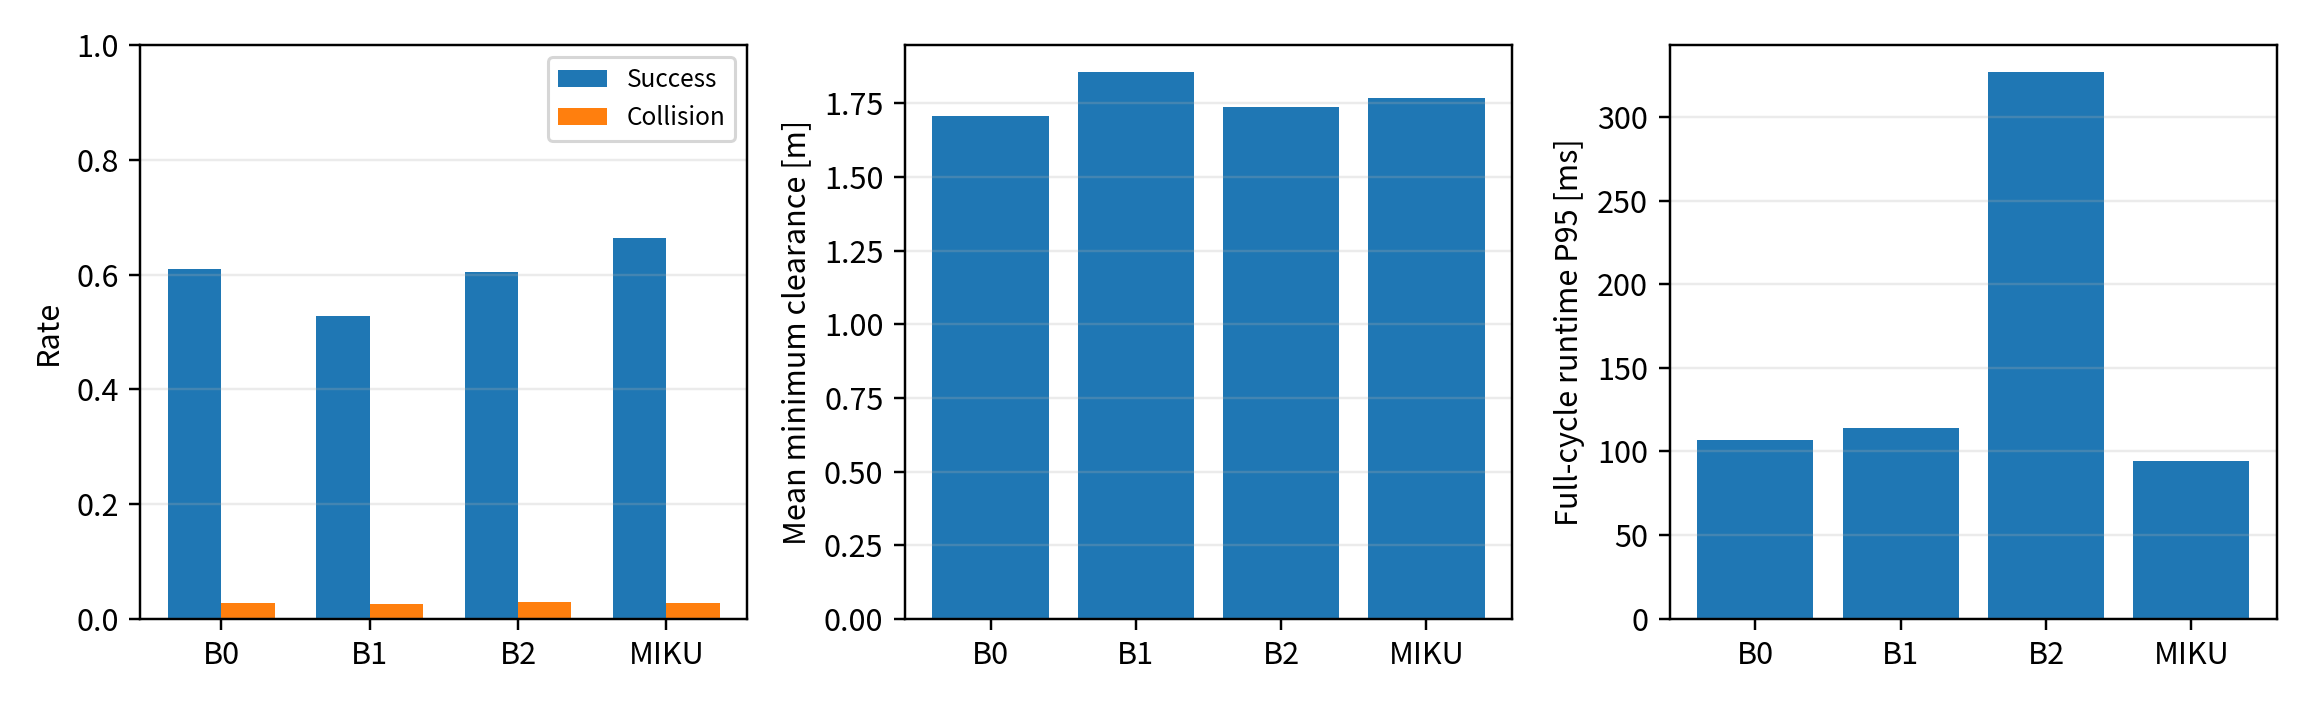
\includegraphics[width=0.96\textwidth]{generated/randomized_summary.png}
\caption{7 类配对随机场景的总体性能}
\label{fig:summary}
\end{figure}

\subsection{分场景结果}

\begin{table}[htbp]
\centering
\caption{MIKU 相对 B0 的分场景无碰撞到达率}
\label{tab:by-family}
\small
\begin{adjustbox}{max width=\textwidth}
\begin{tabular}{lrrrrr}
\toprule
场景 & B0(\%) & MIKU(\%) & 配对差(pp) & 95\% CI & McNemar $p$\\
\midrule
行人横穿 & \RandCrossingBZeroSuccessPct & \RandCrossingMikuSuccessPct & \RandCrossingMikuVsBZeroSuccessDiff & [\RandCrossingMikuVsBZeroSuccessCiLow,\RandCrossingMikuVsBZeroSuccessCiHigh] & \RandCrossingMikuVsBZeroSuccessMcNemarP\\
车辆切入 & \RandCutInBZeroSuccessPct & \RandCutInMikuSuccessPct & \RandCutInMikuVsBZeroSuccessDiff & [\RandCutInMikuVsBZeroSuccessCiLow,\RandCutInMikuVsBZeroSuccessCiHigh] & \RandCutInMikuVsBZeroSuccessMcNemarP\\
停车+对向车 & \RandParkedBZeroSuccessPct & \RandParkedMikuSuccessPct & \RandParkedMikuVsBZeroSuccessDiff & [\RandParkedMikuVsBZeroSuccessCiLow,\RandParkedMikuVsBZeroSuccessCiHigh] & \RandParkedMikuVsBZeroSuccessMcNemarP\\
窄路多障碍 & \RandNarrowBZeroSuccessPct & \RandNarrowMikuSuccessPct & \RandNarrowMikuVsBZeroSuccessDiff & [\RandNarrowMikuVsBZeroSuccessCiLow,\RandNarrowMikuVsBZeroSuccessCiHigh] & \RandNarrowMikuVsBZeroSuccessMcNemarP\\
多动态交织 & \RandInterleavedBZeroSuccessPct & \RandInterleavedMikuSuccessPct & \RandInterleavedMikuVsBZeroSuccessDiff & [\RandInterleavedMikuVsBZeroSuccessCiLow,\RandInterleavedMikuVsBZeroSuccessCiHigh] & \RandInterleavedMikuVsBZeroSuccessMcNemarP\\
预测含噪 & \RandNoiseBZeroSuccessPct & \RandNoiseMikuSuccessPct & \RandNoiseMikuVsBZeroSuccessDiff & [\RandNoiseMikuVsBZeroSuccessCiLow,\RandNoiseMikuVsBZeroSuccessCiHigh] & \RandNoiseMikuVsBZeroSuccessMcNemarP\\
延迟横穿 & \RandDelayedBZeroSuccessPct & \RandDelayedMikuSuccessPct & \RandDelayedMikuVsBZeroSuccessDiff & [\RandDelayedMikuVsBZeroSuccessCiLow,\RandDelayedMikuVsBZeroSuccessCiHigh] & \RandDelayedMikuVsBZeroSuccessMcNemarP\\
\bottomrule
\end{tabular}
\end{adjustbox}
\end{table}

MIKU 在窄路多障碍中提升 \RandNarrowMikuVsBZeroSuccessDiff 个百分点，说明连续分割与差异化裕度能够恢复被贪心边界压缩的空间通道；在延迟横穿中提升 \RandDelayedMikuVsBZeroSuccessDiff 个百分点，体现了先通过/后通过双向 ST 同伦对通行时机的表达能力。预测含噪场景的到达率提升为 \RandNoiseMikuVsBZeroSuccessDiff 个百分点，其碰撞率配对差为 \RandNoiseMikuVsBZeroCollisionDiff 个百分点，验证了鲁棒占据管的安全作用。行人横穿和多动态交织两类已接近饱和，MIKU 与 B0 保持相当成功率。

\subsection{大规模随机消融}

为避免只在少数手工构型中解释模块作用，消融实验复用主实验相同的 7 类、\RandCaseCount 个种子配对，分别关闭：A1 到达时间初始化投影，A2 障碍物分组，A3 Top-K 连续空间同伦，A4 威胁相关裕度，A5 时间同伦图，A6 鲁棒占据管，A7 交替细化。表~\ref{tab:ablation}中的差值均定义为完整 MIKU 减对应消融版本。

\begin{table}[htbp]
\centering
\caption{MIKU 组件的 \RandCaseCount 例配对随机消融}
\label{tab:ablation}
\small
\begin{adjustbox}{max width=\textwidth}
\begin{tabular}{lrrrrr}
\toprule
配置 & 到达率(\%) & 碰撞率(\%) & 完整方法增益(pp) & 95\% CI & McNemar $p$\\
\midrule
完整 MIKU & \AblMikuSuccessPct & \AblMikuCollisionPct & --- & --- & ---\\
A1 无到达时间初始化 & \AblAOneSuccessPct & \AblAOneCollisionPct & \AblMikuVsAOneSuccessDiff & [\AblMikuVsAOneSuccessCiLow,\AblMikuVsAOneSuccessCiHigh] & \AblMikuVsAOneSuccessMcNemarP\\
A2 无纵向分组 & \AblATwoSuccessPct & \AblATwoCollisionPct & \AblMikuVsATwoSuccessDiff & [\AblMikuVsATwoSuccessCiLow,\AblMikuVsATwoSuccessCiHigh] & \AblMikuVsATwoSuccessMcNemarP\\
A3 无 Top-K 空间同伦 & \AblAThreeSuccessPct & \AblAThreeCollisionPct & \AblMikuVsAThreeSuccessDiff & [\AblMikuVsAThreeSuccessCiLow,\AblMikuVsAThreeSuccessCiHigh] & \AblMikuVsAThreeSuccessMcNemarP\\
A4 无威胁相关裕度 & \AblAFourSuccessPct & \AblAFourCollisionPct & \AblMikuVsAFourSuccessDiff & [\AblMikuVsAFourSuccessCiLow,\AblMikuVsAFourSuccessCiHigh] & \AblMikuVsAFourSuccessMcNemarP\\
A5 无时间同伦图 & \AblAFiveSuccessPct & \AblAFiveCollisionPct & \AblMikuVsAFiveSuccessDiff & [\AblMikuVsAFiveSuccessCiLow,\AblMikuVsAFiveSuccessCiHigh] & \AblMikuVsAFiveSuccessMcNemarP\\
A6 无鲁棒占据管 & \AblASixSuccessPct & \AblASixCollisionPct & \AblMikuVsASixSuccessDiff & [\AblMikuVsASixSuccessCiLow,\AblMikuVsASixSuccessCiHigh] & \AblMikuVsASixSuccessMcNemarP\\
A7 无交替细化 & \AblASevenSuccessPct & \AblASevenCollisionPct & \AblMikuVsASevenSuccessDiff & [\AblMikuVsASevenSuccessCiLow,\AblMikuVsASevenSuccessCiHigh] & \AblMikuVsASevenSuccessMcNemarP\\
\bottomrule
\end{tabular}
\end{adjustbox}
\end{table}

Top-K 空间同伦和威胁相关裕度分别贡献 \AblMikuVsAThreeSuccessDiff 与 \AblMikuVsAFourSuccessDiff 个百分点，是恢复窄路空间可行性的主要来源；时间同伦图贡献 \AblMikuVsAFiveSuccessDiff 个百分点，表明动态冲突需要显式的通行次序。关闭鲁棒占据后碰撞率从 \AblMikuCollisionPct\% 增至 \AblASixCollisionPct\%，完整方法的碰撞率配对差为 \AblMikuVsASixCollisionDiff 个百分点（$p=\AblMikuVsASixCollisionMcNemarP$），直接验证了不确定性管的安全收益。交替细化带来 \AblMikuVsASevenSuccessDiff 个百分点增益，而 A1 差异未达显著，说明二阶到达时间主要提供首轮初始化，最终性能来自同伦搜索、QP 验证和反馈细化的共同作用。

\subsection{滚动规划与联合参照}

滚动实验以 0.5\,s 为执行步长循环“规划--执行--更新预测”，每类 100 个种子，共 \ClosedCaseCount 个场景。MIKU 到达率为 \ClosedMikuSuccessPct\%，B0 为 \ClosedBZeroSuccessPct\%，配对提升 \ClosedMikuVsBZeroSuccessDiff 个百分点，95\% CI [\ClosedMikuVsBZeroSuccessCiLow,\ClosedMikuVsBZeroSuccessCiHigh]，McNemar $p=\ClosedMikuVsBZeroSuccessMcNemarP$。两者碰撞率均为 \ClosedMikuCollisionPct\%。这说明语义同伦保持和先行承诺能够把单周期收益延续到连续重规划，同时没有增加碰撞。表~\ref{tab:closed-joint}中的滚动 P95 是每个场景约 20 个规划周期的累计墙钟时间，并非单周期延迟。

B3 联合参照在 $(t,s,l,v,\dot l)$ 网格上同步搜索，并与 MIKU 使用相同的威胁相关裕度和鲁棒预测管。它不使用路径--速度顺序 QP，因此用于检验解耦方法与联合候选搜索的质量--开销关系，而不是作为连续全局最优上界。

\begin{table}[htbp]
\centering
\caption{滚动规划与联合时空参照结果}
\label{tab:closed-joint}
\small
\begin{tabular}{llrrrr}
\toprule
协议 & 方法 & $n$ & 到达率(\%) & 碰撞率(\%) & P95耗时(ms)\\
\midrule
滚动规划 & B0 & \ClosedCaseCount & \ClosedBZeroSuccessPct & \ClosedBZeroCollisionPct & \ClosedBZeroRuntimePninetyfive\\
滚动规划 & MIKU & \ClosedCaseCount & \ClosedMikuSuccessPct & \ClosedMikuCollisionPct & \ClosedMikuRuntimePninetyfive\\
联合参照 & B3 & \JointCaseCount & \JointBThreeSuccessPct & \JointBThreeCollisionPct & \JointBThreeRuntimePninetyfive\\
联合参照 & MIKU & \JointCaseCount & \JointMikuSuccessPct & \JointMikuCollisionPct & \JointMikuRuntimePninetyfive\\
\bottomrule
\end{tabular}
\end{table}

联合参照中，MIKU 与 B3 的到达率差为 \JointMikuVsBThreeSuccessDiff 个百分点，95\% CI [\JointMikuVsBThreeSuccessCiLow,\JointMikuVsBThreeSuccessCiHigh]，McNemar $p=\JointMikuVsBThreeSuccessMcNemarP$；两者在当前样本中的到达率无显著差异。B3 的 P95 为 \JointBThreeRuntimePninetyfive\,ms，MIKU 为 \JointMikuRuntimePninetyfive\,ms。该对照显示，MIKU 以两个凸 QP 和有限同伦候选取得了与联合网格参照相当的可达性，同时将计算开销降低两个数量级。B3 在成功样本上的通行效率更高，说明联合搜索在时间最优性上仍有优势。

\subsection{灵敏度与适用范围}

对五项威胁权重同时施加 $\pm\SensPerturbPct\%$ 扰动并重新归一，安全裕度最大相对偏差为 \SensWorstRelDev\%；4 个代表性场景各运行 \SensTrajectoryTrialCount 条完整轨迹，共 80 条均保持成功，最大横向轨迹偏差为 0.011\,m。结果表明，方法对权重的局部变化稳定，核心收益不依赖单个精确调参点。

本文实验覆盖规划器在环的结构化道路与有界预测扰动，尚未包含真实感知误检、复杂路口规则和车辆执行器误差。该范围不影响本文对同伦候选、凸性保持和配对仿真结果的验证，也明确了下一阶段实车与概率预测实验的接口。
